\section{Cache Optimizations}
\label{sec:cache_opt}

Our cache optimizations for DNN training are based on the sparse nature of the performance critical data (e.g., activations, errors, etc.).  Our approach improves cache performance through a compact representation of cache lines containing only zeroes (a.k.a. \emph{zero cache lines}) in the caches, which helps to avoid  the normal bandwidth and storage costs of zero cache lines. These optimizations enable efficient scaling of model size and training threads.  

Managing zero data at cache line granularity enables implementation of our optimizations through simple and efficient extensions of existing memory systems.  Our current design comprises of mechanisms for achieving the following: (i) compact representation of zero cache lines, (ii) a decoupled cache hierarchy for zero cache lines, and (iii) tracking zero cache lines in the memory system.  We describe these mechanims in the rest of this section.

\begin{figure}[!t]
\centering
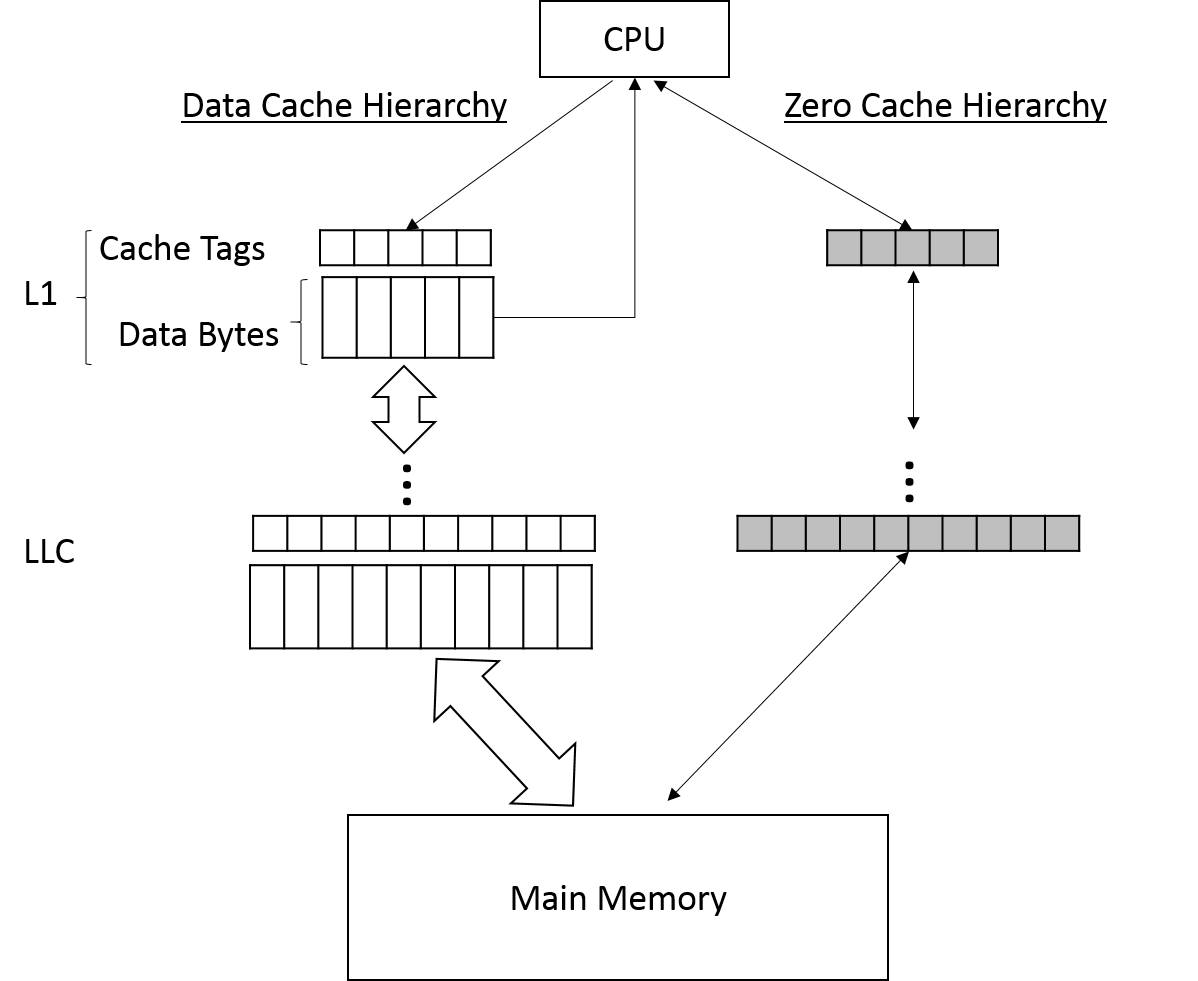
\includegraphics[width=2.4in]{Figures/zero_cache_hierarchy.png}
\caption{A Memory System with Zero Cache Hierarchy.}
\label{fig:zero_cache_hierarchy}
\end{figure}

\subsection{Zero Cache Line Representation}

Our compact representation exploits the fact that the data bytes of a zero cache line are not required to represent the line in cache, the cache tag is sufficient for this purpose. Also, it is not neccesary to transfer the data bytes of a zero cache line across the caches since they can be synthesized in the processor (read) or main memory (on a writeback) as appropriate.  However, in event of a cache hit, we must quickly determine whether it is a zero cache line that is referenced so that the appropriate data transfer is done promptly. We consider two alternatives for handling this: (i) an extra bit in the cache tags to identify zero cache lines, or (ii) a decoupled hierarchy of cache tags for zero cache lines.  Although the first option avoids the extra cost of zero cache line tags, the data bytes space of zero cache lines are unused.  To avoid this waste, we adopt the second option in our current work. 

\begin{figure}[!t]
\centering
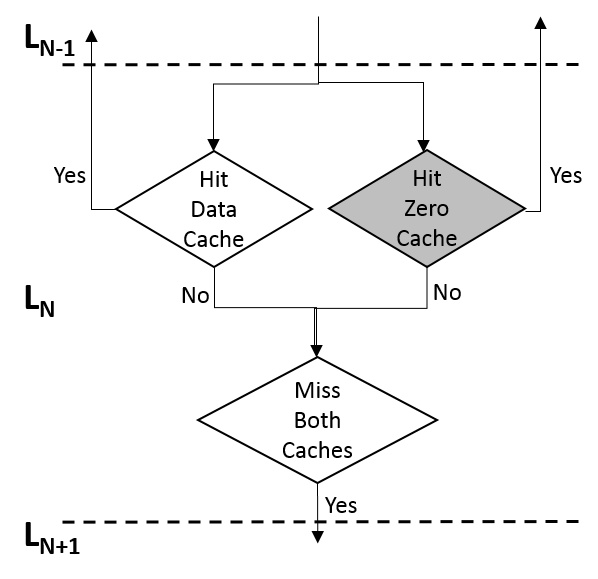
\includegraphics[ height=2in]{Figures/cache_access_flowchart.png}
\caption{Handling read requests.}
\label{fig:cache_access_flowchart}
\end{figure}

\subsection{Hierarchy of Zero Cache Lines}

Figure~\ref{fig:zero_cache_hierarchy} illustrates a memory system that is augmented with a cache hierarchy for zero cache lines, which we call the \emph{zero cache} hierarchy. The zero cache hierarchy is a multi-level structure with caches (a.k.a., \emph{zero caches}) containing tags but no data bytes.  Since zero cache lines are not maintained in the conventional data caches, both cache hierarchies are mutually exclusive. The zero cache hierarchy and the data cache hierarchy have the same number of levels, and can additionally share other properties, such as number of entries, ways, associativity, replacement policies, etc.  The coherence of zero caches is maintained across cores using the same protocol as the data caches. 

Data access requests from the processor are satisfied by accessing the two cache hierarchies in parallel to avoid introducing extra latency. Figure~\ref{fig:cache_access_flowchart} shows the processing of a read request by the $N$th level caches.  The request is processed in parallel by the data  and zero caches, and forwarded to the next level if it is a miss in both.  If the request is a hit in either cache, then the appropriate response is sent to the processor or lower levels of the cache hierarchy.   The data cache responds, as normal, with the requested data bytes (or cache line), while the zero cache responds by signaling a zero cache line hit. 

\begin{figure}[!t]
\centering
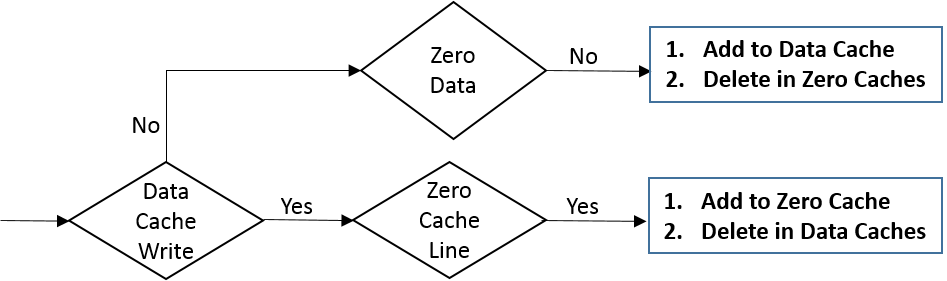
\includegraphics[width=0.9\columnwidth]{Figures/processor_write_flowchart.png}
\caption{Handling processor writes.}
\label{fig:processor_write_flowchart}
\end{figure}

\subsection{Tracking Zero Cache Lines}

Our optimizations are based on the invariant that cache lines reside in the appropriate cache hierarchy: zero cache lines in zero caches and other cache lines in the data caches. To maintain this invariant, we track the zero status of cache lines to ensure that a cache line is placed in the right hierarchy in the following events: (i) update by processor writes, (ii) cache fill from main memory, and (iii) writebacks from lower level caches (e.g., due to evictions). Our tracking operations do not increase cache access latencies as they execute off the critical path of cache accesses. We leverage zero detector hardware~\cite{Dusser09} to detect that an entire cache line (i.e., 32/64 bytes) is zero.

\subsubsection{Processor Writes.}

The zero-status of a cache line can be changed by a processor write depending on the current status and write data.  The following four situations could arise: (i) write zeroes to a zero cache line, (ii) write non-zeroes to a non-zero cache line, (iii) write non-zeroes to a zero cache line, and (iv) write zeroes to a non-zero cache line.  The first two situations are irrelevant since the non-zero status of the cache line is unchanged.  Writing a non-zero value to a zero cache line moves the cache line to the data cache in the the same level, and removes the cache line from the zero cache hierarchy.  This may require data cache evictions to accomodate the new cache line.  Writing zeroes to a non-zero cache line moves the cache line from the data caches into the zero-cache hierarchy if the cache line contains only zeroes after the update.  Naturally, the cache tag is moved as well.  Figure~\ref{fig:processor_write_flowchart} illustrates how cache updates by processor writes are handled to ensure that cache lines reside in the right hierarchy.  

\subsubsection{Cache Fills from Main Memory.} 

Since our optimizations are focused on the cache capacity and bandwidth, the data bytes of zero cache lines are stored in main memory, similar to other cache lines.  We extend the memory controller to avoid sending data bytes when handling a cache fill request for a zero cache line.  Requests for non-zero cache lines are handled normally. 

\subsubsection{Writebacks from Lower Level Caches.}

Our decoupled cache hierarchies approach implicitly handles writebacks from lower level caches because the zero-status of a cache line is unchanged.  Thus, the data caches are not involved by zero cache writebacks, and vice versa.   


